\documentclass[tikz]{standalone}

\usetikzlibrary{calc}

\begin{document}
	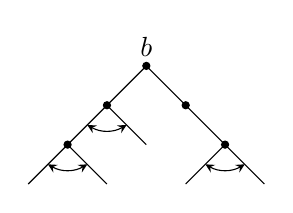
\begin{tikzpicture}[>=stealth,scale=0.5]
	
	\draw (-3,-3) -- (0,0) node [above] {$b$} -- (3,-3);
	
	\draw (-2,-2) -- (-1,-3);
	\draw [<->] ($(-2,-2)!0.5!(-3,-3)$) to [bend right] ($(-2,-2)!0.5!(-1,-3)$);
	
	\draw (-1,-1) to (0,-2);
	\draw [<->] ($(-1,-1)!0.5!(-2,-2)$) to [bend right] ($(-1,-1)!0.5!(0,-2)$);
	
	\draw (2,-2) to (1,-3);
	\draw [<->] ($(2,-2)!0.5!(1,-3)$) to [bend right] ($(2,-2)!0.5!(3,-3)$);
	
	\foreach \x in {
		(0,0),(1,-1),(2,-2),
		(-1,-1),(-2,-2)
	} {
		\fill \x circle (3pt);
	}
	
	\end{tikzpicture}
\end{document}
